
\documentclass{beamer}


\mode<presentation>
{
  \usetheme{CambridgeUS}
	\usecolortheme{beaver}
  % or ...

  \setbeamercovered{transparent}
  % or whatever (possibly just delete it)
}


\usepackage{xeCJK}
\usepackage[english]{babel}
\usepackage[utf8]{inputenc}
\usepackage{times}
\usepackage[T1]{fontenc}
\usepackage{hyperref}
\usepackage{pifont}
\usepackage{bibentry}
\usepackage{verbatim}
\newcommand{\cmark}{\ding{51}}%
\newcommand{\xmark}{\ding{55}}%
\setCJKmainfont{WenQuanYi Micro Hei}


\title[开源软件基础] 
{开源软件基础}
\subtitle{Python Requests}

\author[Zhilei Ren] 
{Zhilei Ren}

\institute[OSCAR Team] % (optional, but mostly needed)
{
\\
\includegraphics[width=0.2\textwidth]{../../utils/logo.jpg}\\
OSCAR Team, School of Software, 
Dalian University of Technology
}


\subject{Open source software}



\pgfdeclareimage[height=0.5cm]{university-logo}{../../utils/logo.jpg}
\logo{\pgfuseimage{university-logo}}



% Delete this, if you do not want the table of contents to pop up at
% the beginning of each subsection:
\AtBeginSubsection[]
{
  \begin{frame}<beamer>{Outline}
    \tableofcontents[currentsection,currentsubsection]
  \end{frame}
}


% If you wish to uncover everything in a step-wise fashion, uncomment
% the following command: 

%\beamerdefaultoverlayspecification{<+->}

\setbeamertemplate{section in toc}[circle]
\setbeamertemplate{items}[circle]
\setbeamertemplate{caption}[numbered]
\setbeamertemplate{bibliography item}{\insertbiblabel}
\setbeamertemplate{bibliography entry title}{}
\setbeamertemplate{bibliography entry journal}{}

\begin{document}

\begin{frame}
  \titlepage
\end{frame}

%\begin{frame}{Outline}
%  \tableofcontents[currentsection,currentsubsection, 
%    hideothersubsections, 
%    sectionstyle=show,
%]
%\end{frame}

\AtBeginSection[]
{
 \begin{frame}<beamer>
 \frametitle{Outline}
 \tableofcontents[currentsection]
 \end{frame}
}
\begin{frame}[t]{HTTP基础知识}
    \begin{block}
        {HTTP}
        \begin{itemize}
            \item GET 向指定的资源发出“显示”请求。使用GET方法应该只用在读取数据，而不应当被用于产生“副作用”的操作中，例如在Web Application中。其中一个原因是GET可能会被网络蜘蛛等随意访问。
            \item HEAD 与GET方法一样，都是向服务器发出指定资源的请求。只不过服务器将不传回资源的本文部分。它的好处在于，使用这个方法可以在不必传输全部内容的情况下，就可以获取其中“关于该资源的信息”（元信息或称元数据）。
        \end{itemize}
    \end{block}
    
\end{frame}

\begin{frame}[t]{HTTP基础知识}
    \begin{block}
        {HTTP}
        \begin{itemize}
            \item POST 向指定资源提交数据，请求服务器进行处理（例如提交表单或者上传文件）。数据被包含在请求本文中。这个请求可能会创建新的资源或修改现有资源，或二者皆有。
            \item PUT 向指定资源位置上传其最新内容。
            \item DELETE 请求服务器删除Request-URI所标识的资源。
            \item TRACE 回显服务器收到的请求，主要用于测试或诊断。
        \end{itemize}
    \end{block}
    
\end{frame}

\begin{frame}[t]{HTTP基础知识}
    \begin{block}
        {HTTP}
        \begin{itemize}
            \item OPTIONS 这个方法可使服务器传回该资源所支持的所有HTTP请求方法。用'*'来代替资源名称，向Web服务器发送OPTIONS请求，可以测试服务器功能是否正常运作。
            \item CONNECT HTTP/1.1协议中预留给能够将连接改为管道方式的代理服务器。通常用于SSL加密服务器的链接（经由非加密的HTTP代理服务器）。
        \end{itemize}
    \end{block}
    
\end{frame}
\begin{frame}[t,fragile]{数据准备}
    \scriptsize
\begin{verbatim}
$head -n 10 robots.txt # from taobao.com/robots.txt

User-agent:  Baiduspider
Allow:  /article
Allow:  /oshtml
Allow:  /wenzhang
Disallow:  /product/
Disallow:  /

User-Agent:  Googlebot
Allow:  /article
Allow:  /oshtml
        
\end{verbatim}
    
\end{frame}

\begin{frame}[t]{数据准备}
	\centering
	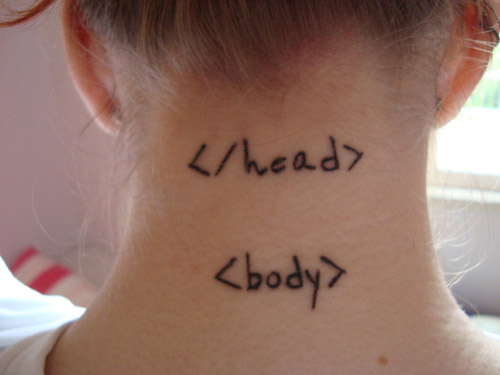
\includegraphics[width=.4\linewidth]{HTML-Tags-Tattoo.jpg}
\end{frame}

\begin{frame}[t,fragile]{数据准备}
    \scriptsize
\begin{verbatim}
$cat index.html # use type in win32
<html>
    <head>
    </head>
    <body>
        <h1>Title</h1>
        <p> This is a paragraph</p>
        <table>
            <tr>
                <td>A11</td> <td>A12</td> <td>A13</td>
            </tr>
            <tr>
                <td>A21</td> <td>A22</td> <td>A23</td>
            </tr>
            <tr>
                <td>A31</td> <td>A32</td> <td>A33</td>
            </tr>
    </body>
</html>

$python3 -m http.server 
Serving HTTP on 0.0.0.0 port 8000 (http://0.0.0.0:8000/) ... 
        
\end{verbatim}
    
\end{frame}

\begin{frame}{本地vs.远程}
    \Huge
    我发起疯来，连自己都爬
    
\end{frame}
\section{Robots协议} % (fold)
\label{sec:Robots协议}
\begin{frame}
  \frametitle{机器人协议}
	robots.txt（统一小写）是一种存放于网站根目录下的ASCII编码的文本文件，它通常告诉网络搜索引擎的漫游器（又称网络蜘蛛），此网站中的哪些内容是不应被搜索引擎的漫游器获取的，哪些是可以被漫游器获取的。因为一些系统中的URL是大小写敏感的，所以robots.txt的文件名应统一为小写。robots.txt应放置于网站的根目录下。如果想单独定义搜索引擎的漫游器访问子目录时的行为，那么可以将自定的设置合并到根目录下的robots.txt，或者使用robots元数据（Metadata，又称元数据）。\footnote{\url{https://zh.wikipedia.org/wiki/Robots.txt}}
\end{frame}

\begin{frame}
  \frametitle{机器人协议}
	\begin{block}
		{协议特点}
		\begin{itemize}
			\item robots.txt协议并不是一个规范，而只是约定俗成的，所以并不能保证网站的隐私。
			\item 用字符串比较来确定是否获取URL，所以目录末尾有与没有斜杠“/”表示的是不同的URL。
			\item 允许使用类似"Disallow: *.gif"这样的通配符。
		\end{itemize}
	\end{block}
\end{frame}

\begin{frame}[t,fragile]
  \frametitle{机器人协议}
	\begin{block}
		{允许所有的机器人：}
\begin{verbatim}
User-agent: *
Disallow:
\end{verbatim}
	\end{block}
	\begin{block}
		{另一写法}
\begin{verbatim}
User-agent: *
Allow:/
\end{verbatim}
	\end{block}
\end{frame}

\begin{frame}[t,fragile]
  \frametitle{机器人协议}
	\begin{block}
		{仅允许特定的机器人：}
\begin{verbatim}
User-agent: name_spider
Allow:
\end{verbatim}
	\end{block}
	\begin{block}
		{拦截所有的机器人}
\begin{verbatim}
User-agent: *
Disallow: /
\end{verbatim}
	\end{block}
\end{frame}

\begin{frame}[t,fragile]
  \frametitle{机器人协议}
	\begin{block}
		{禁止所有机器人访问特定目录}
\begin{verbatim}
User-agent: *
Disallow: /cgi-bin/
Disallow: /images/
Disallow: /tmp/
Disallow: /private/
\end{verbatim}
	\end{block}
	\begin{block}
		{仅禁止坏爬虫访问特定目录}
\begin{verbatim}
User-agent: BadBot
Disallow: /private/
\end{verbatim}
	\end{block}
\end{frame}

\begin{frame}[t,fragile]
  \frametitle{机器人协议}
	\begin{block}
		{禁止所有机器人访问特定目录}
\begin{verbatim}
User-agent: *
Disallow: /*.php$
Disallow: /*.js$
Disallow: /*.inc$
Disallow: /*.css$
\end{verbatim}
	\end{block}
\end{frame}

\begin{frame}
  \frametitle{如何遵守协议}
	\begin{block}
		{}
		\begin{itemize}
			\item 人工阅读robots.txt
			\item 使用urllib.robotparser
		\end{itemize}
	\end{block}
\end{frame}

\begin{frame}[t,fragile]
  \frametitle{解析robots.txt}
	\scriptsize
\begin{verbatim}
>>> import urllib.robotparser
>>> rp = urllib.robotparser.RobotFileParser()
>>> rp.set_url("http://127.0.0.1:8000/robots.txt")
>>> rp.read()
>>> rp.can_fetch("Baiduspider", "http://127.0.0.1:8000/")
False
>>> rp.can_fetch("Baiduspider", "http://127.0.0.1:8000/article/")
True
\end{verbatim}
	
\end{frame}
% section Robots协议 (end)
\section{License} % (fold)
\label{sec:License}


\begin{frame}[t]{Apache2 License}

A large number of open source projects you find today are GPL Licensed.
While the GPL has its time and place, it should most certainly not be your
go-to license for your next open source project.

\end{frame}


\begin{frame}[t]{Apache2 License}

A project that is released as GPL cannot be used in any commercial product
without the product itself also being offered as open source.

\end{frame}


\begin{frame}[t]{Apache2 License}

The MIT, BSD, ISC, and Apache2 licenses are great alternatives to the GPL
that allow your open-source software to be used freely in proprietary,
closed-source software.

Requests is released under terms of Apache2 License.
\end{frame}



% section License (end)
\section{Requests: HTTP for Humans} % (fold)
\label{sec:Requests: HTTP for Humans}



\begin{frame}[t,fragile]{Requests: HTTP for Humans}


\begin{verbatim}


>>> r = requests.get('https://api.github.com/user', auth=('user', 'pass'))
>>> r.status_code
200
>>> r.headers['content-type']
'application/json; charset=utf8'
>>> r.encoding
'utf-8'
>>> r.text
u'{"type":"User"...'
>>> r.json()
{u'private_gists': 419, u'total_private_repos': 77, ...}


\end{verbatim}


\end{frame}


\begin{frame}[t]{Requests: HTTP for Humans}

See similar code, sans Requests.

\end{frame}




\begin{frame}[t]{User Testimonials}

Twitter, Spotify, Microsoft, Amazon, Lyft, BuzzFeed, Reddit, The NSA, Her Majesty's Government, Google, Twilio, Runscope, Mozilla, Heroku,
PayPal, NPR, Obama for America, Transifex, Native Instruments, The Washington
Post, SoundCloud, Kippt, Sony, and Federal U.S.
Institutions that prefer to be unnamed claim to use Requests internally.

\end{frame}


\begin{frame}[t]{User Testimonials}

Requests is one of the most downloaded Python packages of all time, pulling in
over 13,000,000 downloads every month. All the cool kids are doing it!

Requests is ready for today's web.

Requests officially supports Python 2.6–2.7 \& 3.4–3.7, and runs great on PyPy.

\end{frame}

% section Requests: HTTP for Humans (end)
\section{Tutorial} % (fold)
\label{sec:Tutorial}

\begin{frame}[t,fragile]{发起连接}
\begin{verbatim}
import requests
r = requests.get("http://127.0.0.1:8000")
print(r.text)
print(r.encoding)
print(r.url)
print(r.status_code)
\end{verbatim}
    
\end{frame}

\begin{frame}[t,fragile]{GET参数}
    \begin{verbatim}
    import requests
    import json
    payload = {'key1': 'value1', 'key2': 'value2'}
    r = requests.get('http://httpbin.org/get', params=payload)
    result = json.loads(r.text)
    print(result['args'])

    \end{verbatim}

\end{frame}
\begin{frame}[t,fragile]{编码问题}
    \begin{verbatim}
    r = requests.get("http://127.0.0.1:8000")
    r.encoding = "UTF-8"
    print(r.text)
    \end{verbatim}
\end{frame}
\begin{frame}[t,fragile]{POST参数}
    \begin{verbatim}
    >>> r = requests.post('http://httpbin.org/post', data = {'key':'value'})
    \end{verbatim}
\end{frame}
% section Tutorial (end)
\section{使用正规式} % (fold)
\label{sec:使用正规式}

\begin{frame}[t]{正规式}
    \begin{block}
        {正规式}
        正则表达式，又称正规表示式、正规表示法、正规表达式、规则表达式、常规表示法（英语：Regular Expression，在代码中常简写为regex、regexp或RE），是计算机科学的一个概念。正则表达式使用单个字符串来描述、匹配一系列匹配某个句法规则的字符串。在很多文本编辑器里，正则表达式通常被用来检索、替换那些匹配某个模式的文本。\footnote{\url{https://zh.wikipedia.org/zh-cn/正则表达式}}
    \end{block}
    
\end{frame}
\begin{frame}[t,fragile]{正规式}

    \begin{verbatim}
>>> import re
>>> re.findall(r'\bf[a-z]*', 'which foot or hand fell fastest')
['foot', 'fell', 'fastest']
>>> re.sub(r'(\b[a-z]+) \1', r'\1', 'cat in the the hat')
'cat in the hat'
        
    \end{verbatim}
    
\end{frame}

\begin{frame}[t]{匹配字符}

	\begin{block}{特殊字符}
\begin{itemize}
	\item[$\bullet$] [a-z]表示在范围内选择
	\item[$\bullet$] \^{} \$表示位置（首尾），\textbackslash \^{}和\textbackslash \$表示字面值
	\item[$\bullet$] \textbackslash b表示单词边界
	\item[$\bullet$] \textbackslash w表示字母表中任意字符
	\item[$\bullet$] \textbackslash s表示空白符
	\item[$\bullet$] .表示任意字符，\textbackslash .表示点号
\end{itemize}
	\end{block}

\end{frame}

\begin{frame}[t]{模式重复}
	\begin{block}{模式重复}
		\begin{itemize}
			\item *表示出现0次或多次
			\item +表示出现1次或多次
			\item *?和+?表示最短匹配
			\item \{5\}和\{3,6\}表示重复5次/3至6次
			\item ()用于分组，\textbackslash 数字用于引用分组
		\end{itemize}

	\end{block}
\end{frame}

\begin{frame}[t,fragile]{匹配模式}
	\scriptsize
\begin{verbatim}
>>> import re
>>> ret = re.match(r'ab*', 'abbbbbb')
>>> ret.group()
>>> ret = re.match(r'.*href="(.*?)".*', '<a href="../../a.jpg" >abc</a>')
>>> ret.group()
'<a href="../../a.jpg" >abc</a>'
>>> ret.groups()
('../../a.jpg',)
>>> re.match(r'.*href="(.*?)".*', '<a href="../../a.jpg" >abc</a>')
['../../a.jpg']
>>> re.findall(r'(.)\1', '亮亮明明蛋蛋')
['亮', '明', '蛋']

\end{verbatim}
\end{frame}
\begin{frame}[t]{match与findall的区别}
	\begin{itemize}
		\item match需要从首位置匹配串
		\item findall可以匹配子串
		\item 还有一个search，只返回第一个匹配位置
	\end{itemize}
	
\end{frame}
\begin{frame}[t]{正规式的局限性}
	\begin{block}{回顾编译原理}
\begin{itemize}
	\item 正规式无法表达复杂语法结构
	\item 只用于词法分析
	\item 将文本流转换为记号流
	\item 需要语法分析，借助上下文无关文法构造语法树
	\item HTML解析中，当需要知道href字段处于哪个结点时，需要了解DOM树
\end{itemize}
	\end{block}
\end{frame}
\begin{frame}[t,fragile]{DOM树}
	\begin{minipage}
		{0.4\linewidth}
\begin{verbatim}
<html>
  <head>
    <title>
      My title
    </title>
  </head>
  <body>
    <a href="link.html">My link</a>
    <h1>My header</h1>
  </body>
</html>
\end{verbatim}

	\end{minipage}
	\begin{minipage}
		{0.5\linewidth}
		\vspace{-1in}
	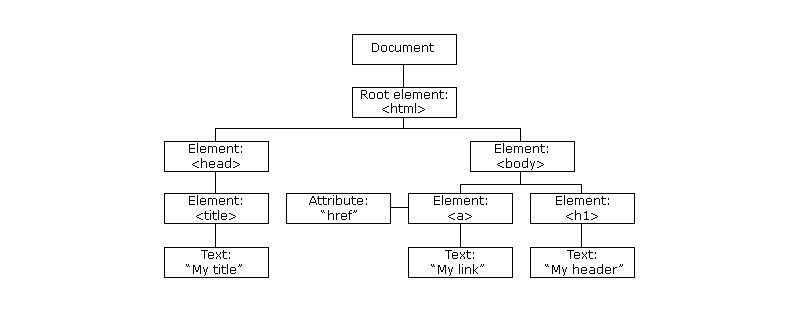
\includegraphics[width=1.3\linewidth]{dom-tree.jpg}
	\end{minipage}
\end{frame}

\begin{frame}[t]{抽象语法树}
	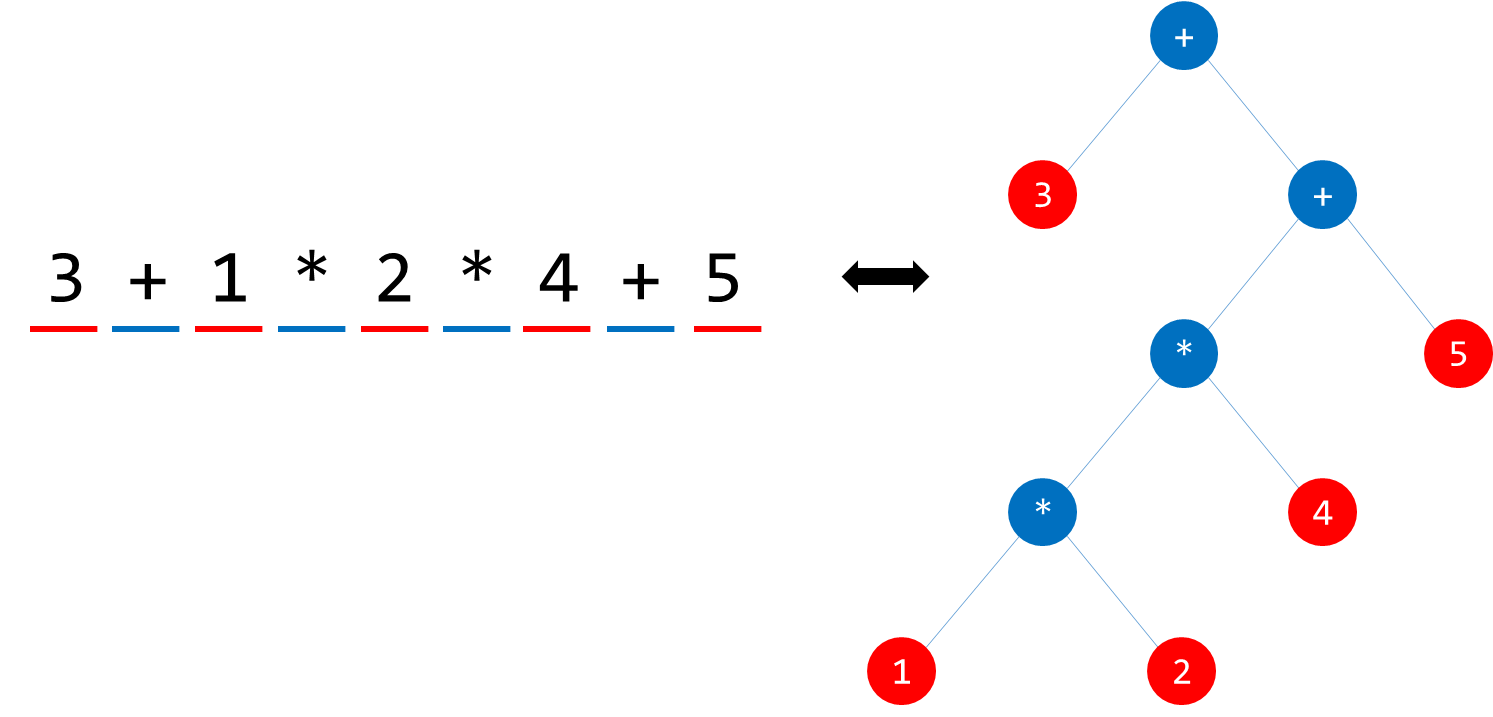
\includegraphics[width=.8\linewidth]{ast.png}
\end{frame}


% section 使用正规式 (end)
\end{document}
